% =====================================================================
%  Narrative--Positioning Divergence (NPD)
%  An Embedding-Based Framework for Contrarian Sentiment and for
%  Forecasting the Market's Interpretation of News
%  Technical Report -- First Draft (v0.1)
% =====================================================================
\documentclass[11pt,a4paper]{article}

% ---------- Packages -------------------------------------------------
\usepackage[utf8]{inputenc}
\IfFileExists{lmodern.sty}{\usepackage[T1]{fontenc}\usepackage{lmodern}}{}
\usepackage[margin=2.5cm]{geometry}
\usepackage{amsmath,amssymb,amsthm,mathtools,bm}
\usepackage{booktabs,tabularx,multirow,array}
\usepackage{enumitem}
\usepackage{graphicx}
\usepackage{xcolor}
\usepackage{algorithm}
\usepackage{algpseudocode}
\usepackage{tikz}
\usetikzlibrary{positioning,arrows.meta,fit,backgrounds,calc}
\usepackage[numbers,sort&compress]{natbib}
\usepackage{microtype}
\usepackage{setspace}
\usepackage[colorlinks=true,linkcolor=blue!50!black,citecolor=blue!50!black,urlcolor=blue!50!black]{hyperref}
\usepackage[capitalise,noabbrev]{cleveref}

\setstretch{1.08}
\setlist{itemsep=2pt,topsep=4pt}

% ---------- Theorem environments ------------------------------------
\theoremstyle{plain}
\newtheorem{proposition}{Proposition}
\newtheorem{corollary}{Corollary}
\newtheorem{lemma}{Lemma}
\theoremstyle{definition}
\newtheorem{definition}{Definition}
\newtheorem{assumption}{Assumption}
\newtheorem{hypothesis}{Hypothesis}
\theoremstyle{remark}
\newtheorem{remark}{Remark}
\crefname{hypothesis}{Hypothesis}{Hypotheses}
\crefname{assumption}{Assumption}{Assumptions}
\crefname{definition}{Definition}{Definitions}

% ---------- Macros ---------------------------------------------------
\newcommand{\R}{\mathbb{R}}
\newcommand{\E}{\mathbb{E}}
\newcommand{\Prob}{\mathbb{P}}
\newcommand{\F}{\mathcal{F}}
\newcommand{\N}{\mathcal{N}}
\newcommand{\z}{\bm{z}}
\newcommand{\w}{\bm{w}}
\newcommand{\x}{\bm{x}}
\newcommand{\ind}{\mathbf{1}}
\DeclareMathOperator*{\argmin}{arg\,min}
\DeclareMathOperator*{\argmax}{arg\,max}
\DeclareMathOperator{\sgn}{sgn}
\DeclareMathOperator{\Var}{Var}
\DeclareMathOperator{\Cov}{Cov}
\DeclareMathOperator{\tr}{tr}
\newcommand{\todo}[1]{\textcolor{red!70!black}{\textbf{[TODO: #1]}}}

% =====================================================================
\title{\textbf{Narrative--Positioning Divergence}\\[4pt]
\large An Embedding-Based Framework for Contrarian Sentiment\\
and for Forecasting the Market's Interpretation of News\\[6pt]
\normalsize Technical Report --- First Draft (v0.1)}
\author{[Author Name]\thanks{Draft for internal review. Not investment advice. No empirical results are reported in this version; all tables of results are templates to be populated under the protocol in \cref{sec:validation}.}}
\date{September 2026}

\begin{document}
\maketitle

% =====================================================================
\begin{abstract}
\noindent
Financial news is usually treated as a signal whose \emph{polarity} predicts returns. We argue that the economically relevant object is instead the \emph{divergence} between three quantities: (i) what the public narrative says, (ii) what informed capital is doing, and (iii) how prices actually absorb the narrative relative to what the narrative implies. We formalise this idea as the \emph{Narrative--Positioning Divergence} (NPD) framework. On the theory side, a stylised price-formation model with a narrative-sensitive fringe and a strategic informed trader shows that (a) narrative overreaction generates contrarian predictability in narrative sentiment, (b) the residual price reaction net of the narrative-implied move (\emph{absorption}) is a sufficient statistic for informed flow and predicts continuation in the absorbed direction, and (c) observed positioning strictly reduces forecast variance. On the representation side, we propose a point-in-time transformer embedding stack with return-aligned contrastive fine-tuning, anisotropy-corrected Matryoshka embeddings, orthogonalised concept directions and sparse-autoencoder features, narrative distributions compared via entropic optimal transport and kernel MMD, Hawkes-process virality, and an \emph{expectation embedding} that yields a Mahalanobis \emph{semantic surprise}. We define the \emph{Market Interpretation Function}, a conditional distribution of abnormal returns given a news embedding and market state, estimated by kernel analog regression, mixture-density networks and a point-in-time retrieval-augmented language model. On the quant side, positioning is filtered from mixed-frequency disclosures with a lag-augmented Kalman state space, microstructure is measured through order-flow imbalance, Kyle's $\lambda$ and square-root impact, and lead--lag between narrative and positioning is captured by path-signature L\'evy areas. Signals are fused through a regime-switching mixture of experts, calibrated with adaptive conformal inference, and translated into positions through a cost-aware, factor-neutral convex optimiser. We close with a pre-registered validation protocol based on combinatorial purged cross-validation, the deflated Sharpe ratio, the probability of backtest overfitting, and superior-predictive-ability tests, together with explicit controls for look-ahead bias in pretrained language models.
\end{abstract}

\noindent\textbf{Keywords:} textual analysis; contrarian sentiment; representation learning; contrastive learning; optimal transport; informed trading; market microstructure; path signatures; conformal prediction; backtest overfitting.\\
\textbf{JEL:} G12, G14, G41, C45, C55, C58.

\tableofcontents
\newpage

% =====================================================================
\section{Introduction}\label{sec:intro}

Market participants frequently observe that bearish headlines cluster near local price lows and bullish headlines near local highs, and many suspect that large institutions amplify fear in order to accumulate at depressed prices. The strong form of this belief, deliberate coordinated deception, is difficult to establish and, where it occurs, is unlawful market manipulation. A weaker and empirically tractable form is far more useful: \emph{the information content of public narrative and the information content of capital allocation can diverge, and the divergence is measurable}.

This report develops a framework that is agnostic about intent. It does not assume that institutions issue false alarms. Instead, it treats every salient narrative event as generated by one of three latent regimes:
\begin{enumerate}[label=(\roman*)]
  \item \textbf{Informational}: the narrative carries fundamental news, informed capital trades in the same direction, and prices drift in the narrative's direction (consistent with post-news drift, \citealp{chan2003}).
  \item \textbf{Overreaction}: the narrative is amplified beyond its fundamental content by attention and sentiment-driven demand \citep{delong1990,barber2008,tetlock2007}, and prices subsequently revert.
  \item \textbf{Strategic}: informed or liquidity-providing capital trades \emph{against} the narrative, possibly exploiting forced or sentiment-driven flow \citep{brunnermeier2005,engelberg2012,kogan2023}.
\end{enumerate}
The inference problem is to compute, in real time and without look-ahead, the posterior probability of each regime and the conditional distribution of subsequent returns.

The second idea in this report is that the object to forecast is not the sentiment of a news item but its \emph{interpretation} by the market. The same headline can move prices in opposite directions depending on what was expected, on current positioning, and on the macro regime \citep{veronesi1999}. We therefore define a \emph{Market Interpretation Function} that maps a news embedding and a market state to a distribution of abnormal returns, and a \emph{semantic surprise} measured relative to an \emph{expected} news embedding rather than relative to zero.

\paragraph{Contributions.}
\begin{enumerate}[label=\textbf{C\arabic*.}]
  \item A stylised model (\cref{sec:theory}) that yields three testable predictions: narrative overreaction implies contrarian predictability; absorption is a sufficient statistic for informed flow; and positioning data strictly reduce forecast variance.
  \item A point-in-time representation-learning stack (\cref{sec:narrative}) with return-aligned contrastive fine-tuning, geometry corrections, interpretable concept directions, and distributional narrative measures based on optimal transport, kernel two-sample statistics, and self-exciting point processes.
  \item A formal treatment of \emph{forecasting the meaning of news} (\cref{sec:interpretation}) through expectation embeddings, semantic surprise, and a Market Interpretation Function with calibrated uncertainty.
  \item A positioning and absorption layer (\cref{sec:positioning,sec:absorption}) combining mixed-frequency Kalman filtering, microstructure measures, square-root impact, and path-signature lead--lag.
  \item A signal-fusion, portfolio and execution layer (\cref{sec:synthesis,sec:portfolio}) and a pre-registered, overfitting-aware validation protocol (\cref{sec:validation}).
\end{enumerate}

% =====================================================================
\section{Related Literature}\label{sec:literature}

\paragraph{Text and returns.} \citet{tetlock2007} shows that media pessimism predicts downward pressure followed by reversion, consistent with noise-trader sentiment. \citet{loughran2011} demonstrate that general-purpose sentiment dictionaries misclassify financial language and provide domain lexicons. \citet{garcia2013} finds that the predictive power of news sentiment concentrates in recessions. \citet{chan2003} documents drift after headline news and reversal after no-news price moves, a distinction our framework nests. \citet{ke2019} develop a supervised sentiment extraction method tailored to return prediction. Transformer-based models such as FinBERT \citep{araci2019} and domain-trained LLMs \citep{wu2023bloomberggpt} improved classification, and \citet{lopezlira2023} show that LLM-derived headline scores predict next-day returns. \citet{glasserman2023} warn that such results may be contaminated by look-ahead bias in pretrained models, a concern central to our design.

\paragraph{Sentiment, attention and limits to arbitrage.} Noise-trader risk \citep{delong1990} and limits to arbitrage \citep{shleifer1997} explain why sentiment can move prices persistently. \citet{baker2006} show that sentiment affects the cross-section most for hard-to-value, hard-to-arbitrage firms. Attention-driven buying \citep{barber2008,da2011} links news salience to demand shocks. \citet{hong1999} unify underreaction and overreaction through heterogeneous, boundedly rational agents.

\paragraph{Informed and strategic trading.} \citet{kyle1985} and \citet{glosten1985} formalise how prices incorporate private information through order flow. \citet{brunnermeier2005} model predatory trading against distressed sellers. \citet{engelberg2012} show that short sellers' advantage comes from superior processing of public news. \citet{cohen2012} separate informative from routine insider trades. \citet{kogan2023} document fraudulent promotional articles and their price effects. Flow toxicity is measured by VPIN \citep{easley2012}, and order-flow imbalance at the top of the book explains short-horizon price changes \citep{cont2014}.

\paragraph{Machine learning in asset pricing.} \citet{gu2020} benchmark ML methods for return prediction; \citet{kelly2024} argue for the virtue of model complexity; \citet{jiang2023} extract signals from price images. Double/debiased machine learning \citep{chernozhukov2018} provides valid inference with high-dimensional nuisance components.

\paragraph{Representation learning.} We build on transformers \citep{vaswani2017}, sentence embeddings \citep{reimers2019}, weakly supervised contrastive embeddings \citep{wang2022e5}, contrastive predictive coding \citep{oord2018}, Matryoshka representations \citep{kusupati2022}, late-interaction retrieval \citep{khattab2020}, low-rank adaptation \citep{hu2022}, retrieval-augmented generation \citep{lewis2020}, topic modelling on embeddings \citep{grootendorst2022}, the linear representation hypothesis \citep{park2023}, and sparse dictionary learning of model features \citep{cunningham2023,bricken2023}.

\paragraph{Statistics of backtests.} Data snooping and multiple testing are addressed by the reality check \citep{white2000}, the SPA test \citep{hansen2005}, the $t>3$ hurdle \citep{harvey2016}, the deflated Sharpe ratio \citep{bailey2014dsr}, the probability of backtest overfitting \citep{bailey2017pbo}, and combinatorial purged cross-validation \citep{lopezdeprado2018}.

% =====================================================================
\section{Theoretical Framework}\label{sec:theory}

We present a deliberately minimal model whose purpose is to pin down signs and sufficient statistics, not to describe markets in full.

\subsection{Setup}

\begin{assumption}[Primitives]\label{ass:primitives}
A single asset has terminal value $v\sim\N(0,\sigma_v^2)$. A public narrative $m = v + \eta$ is released, with $\eta\sim\N(0,\sigma_\eta^2)$ independent of $v$. The noise $\eta$ aggregates honest error, attention amplification and possibly strategic distortion.
\end{assumption}

\begin{assumption}[Price formation]\label{ass:price}
The price is set by a narrative-sensitive fringe plus a linear impact of informed flow:
\begin{equation}
  p = \varphi\, m + \lambda\, x, \qquad \varphi \ge 0,\ \lambda>0, \label{eq:price}
\end{equation}
where $\varphi$ is the \emph{narrative multiplier}. An informed trader who knows $v$ submits $x=\beta(v-p)$ with $\beta>0$.
\end{assumption}

The Bayesian weight that a rational observer of $m$ alone would place on the narrative is
\begin{equation}
  w^\star \coloneqq \frac{\sigma_v^2}{\sigma_v^2+\sigma_\eta^2} = \frac{\Cov(v,m)}{\Var(m)}. \label{eq:wstar}
\end{equation}
The fringe \emph{overreacts} to narrative when $\varphi>w^\star$ and \emph{underreacts} when $\varphi<w^\star$.

Solving the fixed point in \eqref{eq:price} with $x=\beta(v-p)$ gives
\begin{equation}
  p = \frac{\varphi m + \lambda\beta v}{1+\lambda\beta}, \qquad
  r \coloneqq v-p = \kappa\,(v-\varphi m), \qquad \kappa\coloneqq\frac{1}{1+\lambda\beta}\in(0,1). \label{eq:return}
\end{equation}

\subsection{Results}

\begin{proposition}[Narrative overreaction implies contrarian predictability]\label{prop:contrarian}
Under \cref{ass:primitives,ass:price},
\[
  \E[r\mid m] = \kappa\,(w^\star-\varphi)\,m .
\]
Hence the predictive loading of future returns on narrative is negative if and only if $\varphi>w^\star$.
\end{proposition}

\begin{proposition}[Absorption is sufficient for informed flow]\label{prop:absorption}
Define the absorption residual $a\coloneqq p-\varphi m$, the price move net of the narrative-implied move. Then $a=\lambda x=\lambda\beta\, r$, so
\[
  \E[r\mid a, m] = \frac{a}{\lambda\beta}.
\]
Absorption predicts continuation in the direction of the residual: a price that falls \emph{less} than the narrative implies ($a>0$ after $m<0$) predicts positive returns.
\end{proposition}

\begin{proposition}[Positioning reduces forecast variance]\label{prop:positioning}
Suppose the econometrician observes a noisy positioning proxy $\hat x = x+\xi$ with $\xi\sim\N(0,\sigma_\xi^2)$ independent of $(v,\eta)$. Let $\varsigma^2\coloneqq\Var(r\mid m)=\kappa^2\sigma_v^2\sigma_\eta^2/(\sigma_v^2+\sigma_\eta^2)$. Then
\[
  \E[r\mid m,\hat x] = \kappa(w^\star-\varphi)\,\frac{\sigma_\xi^2}{\beta^2\varsigma^2+\sigma_\xi^2}\, m \;+\; \frac{\beta\varsigma^2}{\beta^2\varsigma^2+\sigma_\xi^2}\,\hat x,
\]
\[
  \Var(r\mid m,\hat x) = \varsigma^2\,\frac{\sigma_\xi^2}{\beta^2\varsigma^2+\sigma_\xi^2} < \varsigma^2 \quad\text{whenever } \sigma_\xi^2<\infty .
\]
\end{proposition}
Proofs are in \cref{app:proofs}.

\begin{remark}[Strategic alarms]
If an informed party can shift $\eta$ in the direction opposite to $v$, the effective $\sigma_\eta^2$ rises and $w^\star$ falls. A fringe that does not update its $\varphi$ then overreacts more, which strengthens the contrarian loading in \cref{prop:contrarian}. Crucially, the strategic case is distinguished from pure overreaction by the sign of $\hat x$ relative to $m$ and by timing, which motivates the lead--lag measures of \cref{sec:leadlag}.
\end{remark}

\begin{remark}[Nesting drift and reversal]
When $\varphi<w^\star$ the loading is positive and the model predicts post-news drift, consistent with \citet{chan2003}. The framework therefore does not hard-code contrarianism: the sign is governed by the time-varying, estimable narrative multiplier $\varphi_t$ (\cref{sec:multiplier}).
\end{remark}

\subsection{Empirical implications}\label{sec:implications}
\begin{enumerate}[label=\textbf{I\arabic*.}]
  \item Sorting events on narrative surprise yields reversal when the estimated $\varphi_t$ exceeds the estimated $w^\star_t$, and drift otherwise.
  \item Sorting on absorption $a$ yields continuation in the direction of $a$, and the effect survives conditioning on $m$.
  \item Adding positioning proxies raises out-of-sample $R^2$ and shrinks the loading on $m$ toward zero in proportion to proxy precision.
\end{enumerate}

% =====================================================================
\section{System Overview}\label{sec:overview}

\Cref{fig:architecture} summarises the architecture. The organising principle is \emph{point-in-time} (PIT) integrity: every feature for decision time $t$ is computed only from data whose \emph{publication} timestamp precedes $t$, and every model used at $t$ was trained only on data available before $t$.

\begin{figure}[ht]
\centering
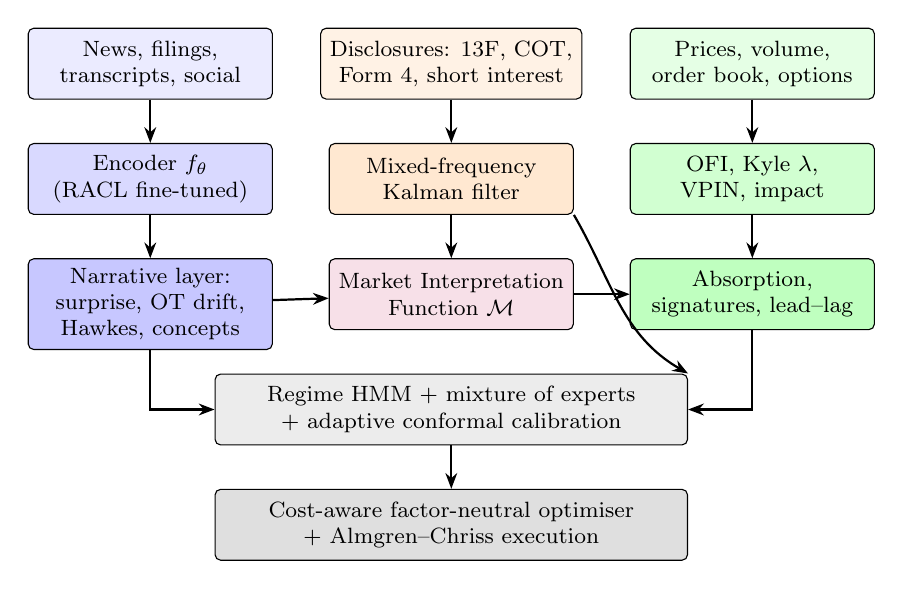
\begin{tikzpicture}[
  node distance=0.55cm and 0.6cm,
  box/.style={draw, rounded corners=2pt, align=center, font=\footnotesize, minimum width=3.1cm, minimum height=0.9cm, fill=#1},
  box/.default=white,
  arr/.style={-{Stealth[length=2mm]}, thick}
]
\node[box=blue!8] (news) {News, filings,\\ transcripts, social};
\node[box=orange!10, right=of news] (pos) {Disclosures: 13F, COT,\\ Form 4, short interest};
\node[box=green!10, right=of pos] (mkt) {Prices, volume,\\ order book, options};

\node[box=blue!15, below=of news] (enc) {Encoder $f_\theta$\\ (RACL fine-tuned)};
\node[box=orange!18, below=of pos] (kf) {Mixed-frequency\\ Kalman filter};
\node[box=green!18, below=of mkt] (micro) {OFI, Kyle $\lambda$,\\ VPIN, impact};

\node[box=blue!22, below=of enc] (narr) {Narrative layer:\\ surprise, OT drift,\\ Hawkes, concepts};
\node[box=purple!12, below=of kf] (mif) {Market Interpretation\\ Function $\mathcal{M}$};
\node[box=green!25, below=of micro] (abs) {Absorption,\\ signatures, lead--lag};

\node[box=gray!15, below=of mif, minimum width=6cm] (hmm) {Regime HMM + mixture of experts\\ + adaptive conformal calibration};
\node[box=gray!25, below=of hmm, minimum width=6cm] (port) {Cost-aware factor-neutral optimiser\\ + Almgren--Chriss execution};

\draw[arr] (news) -- (enc);
\draw[arr] (pos) -- (kf);
\draw[arr] (mkt) -- (micro);
\draw[arr] (enc) -- (narr);
\draw[arr] (micro) -- (abs);
\draw[arr] (narr) -- (mif);
\draw[arr] (kf) -- (mif);
\draw[arr] (mif) -- (abs);
\draw[arr] (narr) |- (hmm);
\draw[arr] (kf.south east) to[out=-60,in=150] (hmm.north east);
\draw[arr] (abs) |- (hmm);
\draw[arr] (hmm) -- (port);
\end{tikzpicture}
\caption{NPD architecture. Three input streams feed a narrative layer, a positioning layer and a microstructure layer. The Market Interpretation Function links narrative to expected price reaction; its residual defines absorption. A regime-switching mixture of experts fuses the layers into calibrated return forecasts.}
\label{fig:architecture}
\end{figure}

\begin{table}[ht]
\centering
\caption{Core notation.}\label{tab:notation}
\small
\begin{tabularx}{\textwidth}{@{}lX@{}}
\toprule
Symbol & Meaning \\
\midrule
$i,\ t,\ h$ & asset index, decision time, forecast horizon \\
$d_j,\ \tau_j$ & document $j$ and its PIT publication timestamp \\
$\z_j\in\R^D$ & embedding of document $j$ from encoder $f_\theta$ \\
$\hat\z_{i,t}$ & expectation embedding: predicted news embedding for $i$ given $\F_{t^-}$ \\
$\bm\varepsilon_{i,t}=\z-\hat\z$ & semantic innovation; $S_{i,t}$ its Mahalanobis magnitude \\
$\w_s^\perp$ & topic-orthogonalised sentiment direction \\
$s_{i,t},\ \tilde s_{i,t}$ & sentiment surprise and its cross-sectionally standardised version \\
$Q_{i,t}$ & narrative distribution: weighted empirical measure of embeddings \\
$\mathcal{M}(\z,\bm\zeta)$ & Market Interpretation Function: law of abnormal returns given news and state \\
$P_{i,t},\ \tilde P_{i,t}$ & filtered latent informed positioning and its standardised version \\
$A_{i,t}$ & standardised absorption (interpretation gap) \\
$\mathcal{L}_{i,t}$ & signature L\'evy area between positioning and negated narrative \\
$\pi_{i,t}(k)$ & filtered posterior probability of regime $k\in\{\mathrm{I},\mathrm{O},\mathrm{S}\}$ \\
$\varphi_t$ & time-varying narrative multiplier \\
\bottomrule
\end{tabularx}
\end{table}

% =====================================================================
\section{Narrative Layer: Representation Learning}\label{sec:narrative}

\subsection{Corpus construction and point-in-time integrity}
The corpus comprises newswire headlines and bodies, regulatory filings, earnings-call transcripts, sell-side note abstracts where licensed, central-bank communications, and social-media posts. Each document receives (i) a PIT timestamp $\tau_j$ equal to first public availability, (ii) entity links to tradable instruments via a named-entity recogniser and a PIT security master, (iii) a source identifier, and (iv) a near-duplicate cluster identifier from MinHash-LSH so that syndicated copies are not double counted.

\subsection{Encoder}
Let $f_\theta:\text{text}\to\R^D$ be a transformer encoder with mean pooling followed by $\ell_2$ normalisation, $\z_j=f_\theta(d_j)/\|f_\theta(d_j)\|$. We initialise from an open-weight embedding model whose pretraining cutoff precedes the evaluation window (\cref{sec:lookahead}) and adapt it with LoRA \citep{hu2022}: each attention projection $W$ is replaced by $W+BA$ with $B\in\R^{D\times r}$, $A\in\R^{r\times D}$, $r\ll D$, which keeps the number of trainable parameters small and reduces the risk of overfitting a finite event sample.

\subsection{Return-aligned contrastive learning (RACL)}
Generic embeddings cluster documents by topic, whereas we need geometry aligned with \emph{economic consequence}. For each training document we form a post-event response vector $\bm\rho_j\in\R^{m}$: abnormal returns over several horizons, abnormal volume, and the change in implied volatility, each cross-sectionally standardised. We define soft positives through a Gaussian kernel on responses,
\begin{equation}
  q_{jk} = \frac{\exp\!\big(-\|\bm\rho_j-\bm\rho_k\|^2/2b^2\big)}{\sum_{l\ne j}\exp\!\big(-\|\bm\rho_j-\bm\rho_l\|^2/2b^2\big)},
\end{equation}
and minimise a soft InfoNCE objective \citep{oord2018} over mini-batches $\mathcal{B}$:
\begin{equation}
  \mathcal{L}_{\mathrm{RACL}} = -\frac{1}{|\mathcal{B}|}\sum_{j\in\mathcal{B}}\sum_{k\ne j} q_{jk}\,
  \log\frac{\exp(\langle\z_j,\z_k\rangle/\tau)}{\sum_{l\ne j}\exp(\langle\z_j,\z_l\rangle/\tau)} .
\end{equation}
To prevent collapse onto return information alone, we add a semantic anchor that distils the frozen encoder's similarity structure,
\begin{equation}
  \mathcal{L}_{\mathrm{anchor}} = \frac{1}{|\mathcal{B}|}\sum_{j}\mathrm{KL}\!\left(\operatorname{softmax}_k\!\big(\langle\z^{(0)}_j,\z^{(0)}_k\rangle/\tau\big)\,\Big\|\,\operatorname{softmax}_k\!\big(\langle\z_j,\z_k\rangle/\tau\big)\right),
\end{equation}
and optimise $\mathcal{L}=\mathcal{L}_{\mathrm{RACL}}+\mu_{\mathrm{a}}\mathcal{L}_{\mathrm{anchor}}$. Because $\bm\rho_j$ contains future information, RACL is trained strictly inside purged training folds (\cref{sec:cpcv}) and re-fitted on a rolling schedule.

\begin{algorithm}[ht]
\caption{Rolling return-aligned contrastive fine-tuning}\label{alg:racl}
\begin{algorithmic}[1]
\Require Documents $\{(d_j,\tau_j,\bm\rho_j)\}$, refit dates $T_1<T_2<\dots$, horizon $H$, embargo $e$
\For{each refit date $T_n$}
  \State $\mathcal{D}_n\gets\{j:\tau_j + H + e < T_n\}$ \Comment{labels fully realised before $T_n$}
  \State Initialise LoRA adapters from $\theta_{n-1}$; freeze base weights
  \For{epoch $=1,\dots,E$}
    \For{mini-batch $\mathcal{B}\subset\mathcal{D}_n$ stratified by date and sector}
      \State Compute $\z_j$, $q_{jk}$; update adapters on $\mathcal{L}_{\mathrm{RACL}}+\mu_{\mathrm{a}}\mathcal{L}_{\mathrm{anchor}}$
    \EndFor
  \EndFor
  \State Freeze $\theta_n$; use it only for documents with $\tau_j\ge T_n$
\EndFor
\end{algorithmic}
\end{algorithm}

\subsection{Embedding geometry}
Transformer embeddings are anisotropic: they occupy a narrow cone, which inflates cosine similarities. We apply PIT whitening,
\begin{equation}
  \bm u_j = \hat\Sigma_{z}^{-1/2}(\z_j-\hat{\bm\mu}_z),
\end{equation}
with $\hat\Sigma_z$ a Ledoit--Wolf shrinkage estimator \citep{ledoit2004} fitted on trailing data. Matryoshka training \citep{kusupati2022} supplies nested prefixes $\z_{[:64]}\subset\z_{[:256]}\subset\z_{[:D]}$, used respectively for fast candidate retrieval in an HNSW index, for density estimation, and for final scoring. Where token-level evidence matters, for instance in long transcripts, we use late-interaction scoring \citep{khattab2020} between query phrases and document tokens.

\subsection{Concept directions and interpretable features}
Following the linear representation hypothesis \citep{park2023}, we estimate concept directions for sentiment, uncertainty, urgency (``alarm''), hedging language, capitulation vocabulary and institutional versus retail register. For concept $c$ with labelled contrast sets $\mathcal{C}^+_c,\mathcal{C}^-_c$ we take the ridge-regularised linear probe
\begin{equation}
  \w_c = \argmin_{\w}\sum_{j}\big(y^{c}_j-\langle\w,\bm u_j\rangle\big)^2+\gamma_c\|\w\|^2 .
\end{equation}
Sentiment directions are confounded by topic: bad news in energy and bad news in banking point in different directions. Let $U\in\R^{D\times K}$ collect the leading principal components of sector-topic centroids. We orthogonalise,
\begin{equation}
  \w_s^\perp = (I-UU^\top)\,\w_s,
\end{equation}
so that sentiment scores are comparable across topics. To discover concepts that are not pre-specified, we train a sparse autoencoder \citep{cunningham2023,bricken2023} on whitened embeddings,
\begin{equation}
  \bm h=\mathrm{ReLU}\big(W_e(\bm u-\bm b_d)+\bm b_e\big),\quad
  \hat{\bm u}=W_d\bm h+\bm b_d,\quad
  \mathcal{L}_{\mathrm{SAE}}=\|\bm u-\hat{\bm u}\|_2^2+\lambda_1\|\bm h\|_1,
\end{equation}
with an overcomplete dictionary. Active dictionary features are named by inspecting top-activating documents and are screened for predictive content only inside training folds.

\subsection{Narratives as distributions}
A narrative is not a single document but a distribution of documents. For asset $i$ at time $t$ we define the decayed empirical measure
\begin{equation}
  Q_{i,t} = \sum_{j:\,\tau_j<t,\ j\to i} \omega_j\,\delta_{\bm u_j},\qquad
  \omega_j\propto c_{\mathrm{src}(j)}\,e^{-(t-\tau_j)/T_{1/2}\cdot\ln 2},
\end{equation}
where $c_{\mathrm{src}}$ is a source credibility weight (\cref{sec:credibility}). We measure narrative drift with the entropic optimal-transport cost \citep{cuturi2013}
\begin{equation}
  W_\epsilon(Q_{i,t},Q_{i,t-\Delta}) = \min_{\bm\Pi\in\Pi(Q_{i,t},Q_{i,t-\Delta})}\langle\bm\Pi,C\rangle-\epsilon H(\bm\Pi),\qquad C_{jk}=\|\bm u_j-\bm u_k\|^2,
\end{equation}
and test for narrative regime breaks with the unbiased kernel MMD statistic \citep{gretton2012},
\begin{equation}
  \widehat{\mathrm{MMD}}^2_k = \E k(\bm u,\bm u')+\E k(\bm u^\ast,\bm u^{\ast\prime})-2\,\E k(\bm u,\bm u^\ast),
\end{equation}
calibrated by permutation. Narrative novelty for a single document is the mean cosine distance to its $k$ nearest neighbours in a PIT memory bank, $\nu(\z_j)=k^{-1}\sum_{l\in\mathrm{kNN}(j)}(1-\langle\z_j,\z_l\rangle)$.

\subsection{Virality and coordination: self-exciting arrivals}
Document arrivals within a semantic cluster $g$ are modelled as a Hawkes process \citep{hawkes1971,bacry2015},
\begin{equation}
  \lambda_g(t)=\mu_g+\sum_{\tau_j<t,\ j\in g}\alpha_g\, e^{-\beta_g(t-\tau_j)},\qquad n_g=\alpha_g/\beta_g,
\end{equation}
where the branching ratio $n_g$ measures the share of documents triggered by earlier documents rather than by exogenous events. A narrative with high $n_g$, low novelty, few independent sources and large reach is \emph{amplified} rather than \emph{informed}; this pattern is an input to the overreaction and strategic regimes. Neural Hawkes variants \citep{mei2017} are a later extension.

\subsection{Source credibility}\label{sec:credibility}
For each source $\mathrm{src}$ we maintain a Beta posterior over its directional hit rate: after each resolved event, $\mathrm{Beta}(a,b)$ is updated with $a\mathrel{+}=\ind\{\sgn(s_j)=\sgn(\mathrm{CAR}_j)\}$ and $b\mathrel{+}=1-\ind\{\cdot\}$. The credibility weight is the posterior mean shrunk toward the population mean. Sources whose hit rate is reliably \emph{below} one half are informative in reverse; their sign is retained and their contribution enters the contrarian channel explicitly rather than being discarded.

% =====================================================================
\section{Forecasting the Market's Interpretation of News}\label{sec:interpretation}

\subsection{Expectation embeddings and semantic surprise}
Markets price the \emph{unexpected} part of news. We therefore forecast what the news will say before it arrives. Let $g_\psi$ be a causal sequence model (a small transformer over the last $L$ document embeddings for asset $i$, concatenated with a market-state vector $\bm\zeta_{i,t}$ comprising recent returns, implied volatility, consensus revisions and scheduled-event flags). It is trained with a contrastive predictive objective,
\begin{equation}
  \mathcal{L}_{\mathrm{CPC}}=-\E\log\frac{\exp\big(\langle\hat\z_{i,t},\z^{+}\rangle/\tau\big)}{\sum_{\z'\in\{\z^+\}\cup\mathcal{N}}\exp\big(\langle\hat\z_{i,t},\z'\rangle/\tau\big)},\qquad \hat\z_{i,t}=g_\psi(\z_{i,<t},\bm\zeta_{i,t}),
\end{equation}
where $\z^+$ is the realised next document and $\mathcal{N}$ are negatives from other assets and dates. The semantic innovation and its magnitude are
\begin{equation}
  \bm\varepsilon_{i,t}=\bm u_{i,t}-\hat{\bm u}_{i,t},\qquad S_{i,t}=\bm\varepsilon_{i,t}^\top\hat\Sigma_\varepsilon^{-1}\bm\varepsilon_{i,t},
\end{equation}
and the \emph{directional} sentiment surprise is the projection of the innovation on the topic-orthogonal sentiment direction,
\begin{equation}
  s_{i,t}=\frac{\langle\w_s^\perp,\bm\varepsilon_{i,t}\rangle}{\|\w_s^\perp\|}. \label{eq:surprise}
\end{equation}
This separates \emph{what is new} from \emph{what is negative}. A strongly negative but fully anticipated headline has large $|\langle\w_s^\perp,\bm u\rangle|$ but small $|s|$.

\subsection{The Market Interpretation Function}
\begin{definition}[Market Interpretation Function]
For news embedding $\z$ and state $\bm\zeta$, $\mathcal{M}(\z,\bm\zeta)$ is the conditional law of the abnormal return over the reaction window $[0,\bar\tau]$, $\mathrm{AR}_{[0,\bar\tau]}\mid(\z,\bm\zeta)$. We write $\mu_{\mathcal M}$ and $\sigma_{\mathcal M}$ for its mean and scale.
\end{definition}

We estimate $\mathcal{M}$ with three complementary learners.

\paragraph{(a) Kernel analog regression.} An interpretable nonparametric baseline that asks how the market reacted to semantically similar news in similar states:
\begin{equation}
  \hat\mu_{\mathcal M}(\z,\bm\zeta)=\frac{\sum_{j\in\mathcal{H}_t}k_j\,\mathrm{AR}_j}{\sum_{j\in\mathcal{H}_t}k_j},\qquad
  k_j=K_h(\z,\z_j)\,K_b(\bm\zeta,\bm\zeta_j)\,e^{-(t-\tau_j)/T_a},
\end{equation}
where $\mathcal{H}_t$ contains only events whose reaction window closed before $t$, and $K_h$ is the von Mises--Fisher kernel on the sphere, $K_h(\z,\z')=\exp(\langle\z,\z'\rangle/h)$. Candidate neighbours are retrieved from the HNSW index using Matryoshka prefixes.

\paragraph{(b) Mixture density network.} A neural head on $(\z,\hat\z,\bm\varepsilon,\bm\zeta)$ outputs the mixture density
\[
  p(\mathrm{AR}\mid\cdot)=\textstyle\sum_{c=1}^{C}\pi_c\,\N(\mu_c,\sigma_c^2),
\]
trained by negative log-likelihood and evaluated by the continuous ranked probability score. Multimodality matters: the same news can be read as ``bad for earnings'' or ``good because it forces policy easing'', and a mixture represents both readings.

\paragraph{(c) Retrieval-augmented reasoning.} A PIT-restricted language model receives the new document, the $k$ nearest historical analogues with their realised reactions, and a structured summary of $\bm\zeta$, and returns a probability distribution over reaction buckets together with a short rationale \citep{lewis2020}. Its output enters the ensemble only as a feature, and its value is established by ablation.

\subsection{Look-ahead bias in pretrained language models}\label{sec:lookahead}
A pretrained model may have memorised outcomes that occurred after an event, which silently inflates backtests \citep{glasserman2023}. Controls:
\begin{enumerate}[label=(\roman*)]
  \item \textbf{Cutoff discipline.} Use frozen open-weight snapshots whose training cutoff precedes each test window; report results separately for pre-cutoff and post-cutoff periods.
  \item \textbf{Anonymisation.} Replace company names, tickers, people and dates with placeholders, and re-run the pipeline. A large performance drop indicates memorisation rather than understanding.
  \item \textbf{Memorisation probes.} Ask the model to complete post-event facts (e.g.\ subsequent price level). Above-chance accuracy on held-out probes flags contamination.
  \item \textbf{Temporal fine-tuning.} Every fine-tuned component is refitted on a rolling schedule (\cref{alg:racl}), never on the full sample.
\end{enumerate}

\subsection{The narrative multiplier}\label{sec:multiplier}
\Cref{prop:contrarian} makes the sign of predictability depend on $\varphi_t-w^\star_t$. We estimate the \emph{contemporaneous} reaction coefficient with a time-varying-parameter regression,
\begin{equation}
  \mathrm{AR}_{i,[0,\bar\tau]}=\varphi_t\, s_{i,t}+e_{i,t},\qquad \varphi_t=\varphi_{t-1}+\nu_t,
\end{equation}
filtered by a Kalman filter (\cref{app:kalman}), and the \emph{fundamental} weight $w^\star_t$ by regressing subsequent fundamental outcomes (earnings surprises, estimate revisions) on $s_{i,t}$ over trailing resolved events. The gap $\hat\varphi_t-\hat w^\star_t$ is a regime feature: positive values favour reversal, negative values favour drift.

% =====================================================================
\section{Positioning Layer}\label{sec:positioning}

\subsection{Data and publication lags}
\begin{table}[ht]
\centering
\caption{Positioning sources. Publication lag must be respected in PIT feature construction.}\label{tab:positioning}
\small
\begin{tabularx}{\textwidth}{@{}lllX@{}}
\toprule
Source & Frequency & Typical lag & Content \\
\midrule
13F holdings & Quarterly & up to 45 days & Long equity holdings of large managers \\
COT reports & Weekly & as of Tue., released Fri. & Futures positioning by trader category \\
Form 4 & Event & within 2 business days & Insider transactions \\
Short interest & Twice monthly & several days & Aggregate short positions \\
ETF and fund flows & Daily & 1 day & Creation/redemption, net flows \\
Options & Intraday/daily & real time & Volume, open interest, skew, signed flow \\
Off-exchange volume & Daily/weekly & 0--2 weeks & Share of volume away from lit venues \\
\bottomrule
\end{tabularx}
\end{table}

\subsection{Mixed-frequency state-space filtering}
Let $P_{i,t}$ be the latent informed net demand for asset $i$ at daily frequency, driven by a common factor and an idiosyncratic component,
\begin{align}
  P_{i,t}&=\bm\Lambda_i^\top\bm F_t+p_{i,t}, & p_{i,t}&=\rho_i\,p_{i,t-1}+\eta_{i,t}, & \bm F_t&=\Phi\,\bm F_{t-1}+\bm\upsilon_t .
\end{align}
Each source $k$ provides an observation of the state at a lagged date,
\begin{equation}
  y^{(k)}_{i,t}=h_k\,P_{i,t-\ell_k}+\epsilon^{(k)}_{i,t},\qquad \text{observed only if } t\in\mathcal{T}_k,
\end{equation}
where $\mathcal{T}_k$ is the release calendar and $\ell_k$ the as-of lag. We augment the state with $L=\max_k\ell_k$ lags so that lagged observations enter a linear measurement equation. The Kalman filter skips the update step when no observation is released, which handles mixed frequencies natively. The output is a filtered mean $\hat P_{i,t\mid t}$ and variance, whose inverse provides the precision weight $\sigma_\xi^{-2}$ of \cref{prop:positioning}.

\subsection{Microstructure measures}
\paragraph{Order-flow imbalance.} At top-of-book update $n$ with best bid/ask prices $P^B_n,P^A_n$ and sizes $q^B_n,q^A_n$ \citep{cont2014},
\begin{equation}
  e_n=\ind\{P^B_n\ge P^B_{n-1}\}q^B_n-\ind\{P^B_n\le P^B_{n-1}\}q^B_{n-1}-\ind\{P^A_n\le P^A_{n-1}\}q^A_n+\ind\{P^A_n\ge P^A_{n-1}\}q^A_{n-1},
\end{equation}
aggregated to $\mathrm{OFI}_{i,[t_1,t_2]}=\sum_{n}e_n$.

\paragraph{Kyle's lambda.} Over intraday buckets, $\Delta p_{b}=\lambda_{i,t}\,Q_b+u_b$ with signed volume $Q_b$ from bulk volume classification; $\hat\lambda_{i,t}$ enters \cref{prop:absorption} as the impact scale.

\paragraph{Flow toxicity.} VPIN \citep{easley2012} over volume buckets measures the probability that liquidity providers face informed flow.

\subsection{Options-implied positioning}
From the options surface we extract the 25-delta risk reversal $\mathrm{RR}_{25}=\sigma^{\mathrm{IV}}_{25\Delta\text{C}}-\sigma^{\mathrm{IV}}_{25\Delta\text{P}}$, the implied--realised variance spread, the put/call open-interest ratio and delta-weighted signed options flow. A bearish narrative accompanied by call-side accumulation and a \emph{falling} put skew is a positioning divergence.

% =====================================================================
\section{Absorption and Lead--Lag}\label{sec:absorption}

\subsection{Absorption as an interpretation gap}
\Cref{prop:absorption} identifies absorption as the price move net of the narrative-implied move. Empirically, the narrative-implied move is $\mu_{\mathcal M}$:
\begin{equation}
  A_{i,t}=\frac{\mathrm{AR}_{i,[0,\bar\tau]}-\hat\mu_{\mathcal M}(\z_{i,t},\bm\zeta_{i,t})}{\hat\sigma_{\mathcal M}(\z_{i,t},\bm\zeta_{i,t})} .
\end{equation}
The \emph{opposition} components, positive when evidence runs against the narrative, are
\begin{equation}
  O^{A}_{i,t}=-\sgn(s_{i,t})\,A_{i,t},\qquad O^{P}_{i,t}=-\sgn(s_{i,t})\,\tilde P_{i,t}.
\end{equation}

\subsection{Effort versus result: square-root impact}
Under the square-root law \citep{bouchaud2018}, a metaorder of size $Q$ moves price by approximately $Y\sigma_i\sqrt{Q/V_i}$, with $\sigma_i$ daily volatility, $V_i$ daily volume and $Y=O(1)$. Given abnormal signed volume $Q^{\mathrm{ab}}_{i,t}$ in the narrative direction, the absorption intensity
\begin{equation}
  \Psi_{i,t}=\frac{Y\,\sigma_i\sqrt{|Q^{\mathrm{ab}}_{i,t}|/V_i}}{|\mathrm{AR}_{i,[0,\bar\tau]}|+\epsilon}
\end{equation}
compares expected impact with realised impact. $\Psi\gg1$ means heavy narrative-driven selling produced little price damage, which requires an opposing absorber.

\subsection{Lead--lag via path signatures}\label{sec:leadlag}
For a two-dimensional path $(X_u,Y_u)_{u\in[a,b]}$, the signed L\'evy area is
\begin{equation}
  \mathcal{A}(X,Y)=\tfrac12\int_a^b (X_u-X_a)\,dY_u-(Y_u-Y_a)\,dX_u,
\end{equation}
which is positive when moves in $X$ tend to precede same-direction moves in $Y$. It is the antisymmetric part of the level-two signature \citep{chevyrev2016} and is invariant to time reparametrisation. We define the \emph{strategic lead--lag}
\begin{equation}
  \mathcal{L}_{i,t}=\mathcal{A}\big(\tilde P_{i,\cdot},\,-\tilde s_{i,\cdot}\big)\Big|_{[t-\Delta,\,t]},
\end{equation}
which is positive when positioning moved first and the narrative subsequently moved \emph{against} it, the signature of accumulation ahead of a bearish narrative. Truncated signatures of the joint path $(t,\tilde s,\tilde P,\log\text{price},\text{volume})$ at depth 3 are also passed to the learners as order-aware features. As a nonparametric cross-check, we compute transfer entropy \citep{schreiber2000} from positioning to narrative.

% =====================================================================
\section{Signal Synthesis}\label{sec:synthesis}

\subsection{The Contrarian Divergence Index}
We first define a transparent composite that nests reversal and drift:
\begin{equation}
  \mathrm{CDI}_{i,t}=-\sgn(s_{i,t})\;g\big(|\tilde s_{i,t}|\big)\;\big(\omega_A O^{A}_{i,t}+\omega_P O^{P}_{i,t}+\omega_L\mathcal{L}_{i,t}+\omega_\varphi(\hat\varphi_t-\hat w^\star_t)\big),
\end{equation}
with $g(x)=\tanh(\kappa_g(x-c)_+)$ activating only for sufficiently extreme narrative surprise. If the bracket is positive, the index trades \emph{against} the narrative; if evidence confirms the narrative, the bracket turns negative and the index trades \emph{with} it. Weights are fitted on training folds by penalised rank regression on forward returns.

\subsection{Regime inference}
Let $\bm o_{i,t}=(\tilde s,S,A,\tilde P,\mathcal{L},\Psi,n_g,\hat\varphi-\hat w^\star)_{i,t}$. A three-state hidden Markov model \citep{hamilton1989} with states $k\in\{\mathrm{I},\mathrm{O},\mathrm{S}\}$ has Gaussian emissions $\bm o\mid k\sim\N(\bm m_k,\Sigma_k)$ and a sticky transition matrix. States are identified by sign restrictions on emission means:
\begin{itemize}
  \item $\mathrm{I}$: $\E[\tilde s\,\tilde P]>0$ and $\E[\tilde s\,A]\ge0$ (capital and price confirm the narrative);
  \item $\mathrm{O}$: high $n_g$, low $\Psi$, $\E[\tilde s\,\tilde P]\approx0$ (amplified narrative, no informed opposition);
  \item $\mathrm{S}$: $\E[\tilde s\,\tilde P]<0$, $\E[\mathcal{L}]>0$, high $\Psi$ (informed opposition that leads the narrative).
\end{itemize}
Only \emph{filtered} probabilities $\pi_{i,t}(k)=\Prob(k\mid\bm o_{i,1:t})$ from the forward recursion are used; smoothed probabilities use future data and are forbidden. We call $\pi_{i,t}(\mathrm{S})$ the \emph{Strategic Alarm Probability}.

\subsection{Mixture of experts and stacking}
Each regime has its own expert $f_k$ (gradient-boosted trees and a small MLP on the full feature set $\x_{i,t}$), and the forecast is
\begin{equation}
  \hat r_{i,t+h}=\sum_{k}\pi_{i,t}(k)\,f_k(\x_{i,t}).
\end{equation}
The mixture, the CDI and the kernel-analog forecast are combined by non-negative stacking on out-of-fold predictions. Inference on the marginal contribution of narrative variables uses double/debiased ML \citep{chernozhukov2018} with cross-fitting and the remaining features as nuisance controls.

\subsection{Calibrated uncertainty}
Forecast intervals use adaptive conformal inference \citep{gibbs2021,angelopoulos2021}, which maintains long-run coverage under distribution shift. With target miscoverage $\alpha$ and step $\gamma$,
\begin{equation}
  \alpha_{t+1}=\alpha_t+\gamma\big(\alpha-\mathrm{err}_t\big),\qquad \mathrm{err}_t=\ind\{r_t\notin\hat C_t(\alpha_t)\}.
\end{equation}
Interval width feeds position sizing and the Black--Litterman confidence matrix below.

% =====================================================================
\section{Portfolio Construction and Execution}\label{sec:portfolio}

\subsection{From forecasts to alphas}
Following \citet{grinold2000}, cross-sectional scores are converted to alphas via $\alpha_i=\mathrm{IC}\cdot\sigma_i\cdot\mathrm{score}_i$, with IC estimated out of sample and shrunk toward zero. Alternatively, signal views are blended with equilibrium returns $\bm\Pi$ through Black--Litterman \citep{black1992},
\begin{equation}
  \bm\mu_{\mathrm{BL}}=\big[(\tau\Sigma)^{-1}+\bm P^\top\Omega^{-1}\bm P\big]^{-1}\big[(\tau\Sigma)^{-1}\bm\Pi+\bm P^\top\Omega^{-1}\bm Q\big],
\end{equation}
with $\Omega$ diagonal and proportional to squared conformal interval widths, so that uncertain views receive less weight.

\subsection{Optimisation}
Positions solve the convex programme
\begin{equation}
\begin{aligned}
  \max_{\w}\quad & \bm\alpha^\top\w-\frac{\gamma}{2}\w^\top\hat\Sigma\w-\sum_i c_i|w_i-w_i^0|-\sum_i\eta_i\,\sigma_i\frac{|w_i-w_i^0|^{3/2}}{\sqrt{V_i}}\\
  \text{s.t.}\quad & B^\top\w=\bm 0,\quad \bm 1^\top\w=0,\quad |w_i|\le\bar w_i,\quad \|\w\|_1\le G,
\end{aligned}
\end{equation}
where $\hat\Sigma$ is a shrinkage covariance \citep{ledoit2004}, the linear term captures spreads and fees, the $3/2$-power term integrates square-root impact, and $B$ contains exposures to market, size, value, profitability, investment and momentum \citep{fama2015,carhart1997} so that the book is neutral to known factors. Hierarchical risk parity \citep{lopezdeprado2016} is a robustness alternative.

\subsection{Sizing}
With estimated edge $\mu$ and variance $\sigma^2$, the growth-optimal fraction is $f^\star=\mu/\sigma^2$ \citep{kelly1956}. Because $\mu$ is estimated with error, we use a fractional Kelly $f=c\,f^\star$ with $c\in[0.25,0.5]$ and cap gross exposure by a CVaR budget.

\subsection{Execution}
Parent orders are scheduled with Almgren--Chriss \citep{almgren2001}. In the continuous-time limit the optimal holdings trajectory is $X(t)=X_0\,\sinh(\kappa(T-t))/\sinh(\kappa T)$ with $\kappa=\sqrt{\lambda_{\mathrm{risk}}\sigma^2/\eta}$, where $\eta$ is the temporary-impact coefficient. Contrarian entries tend to trade against prevailing flow and are therefore naturally liquidity-providing; we exploit this by using passive limit orders during high-$\Psi$ episodes.

% =====================================================================
\section{Validation Protocol}\label{sec:validation}

\subsection{Pre-registered hypotheses}
\begin{hypothesis}[Reversal]\label{hyp:reversal}
Conditional on $|\tilde s|$ in the top decile, $\hat\varphi-\hat w^\star>0$, and $O^P\ge0$, the mean $\mathrm{CAR}_{[1,h]}$ has sign opposite to $s$ for $h\in\{5,20,60\}$ trading days.
\end{hypothesis}
\begin{hypothesis}[Absorption]\label{hyp:absorption}
Controlling for $s$, the coefficient on $A$ in a regression of $\mathrm{CAR}_{[1,h]}$ is positive.
\end{hypothesis}
\begin{hypothesis}[Lead--lag]\label{hyp:leadlag}
Among extreme-narrative events, those with $\mathcal{L}>0$ earn higher contrarian returns than those with $\mathcal{L}\le0$.
\end{hypothesis}
\begin{hypothesis}[Representation]\label{hyp:representation}
Semantic surprise from RACL embeddings has higher out-of-sample predictive accuracy than dictionary \citep{loughran2011}, FinBERT \citep{araci2019} and zero-shot LLM scores \citep{lopezlira2023}.
\end{hypothesis}
\begin{hypothesis}[Economic significance]\label{hyp:economic}
The net-of-cost, factor-neutral portfolio has deflated Sharpe ratio above 0.95 and probability of backtest overfitting below 0.2.
\end{hypothesis}

\subsection{Event-study design}
Abnormal returns are $\mathrm{AR}_{i,\tau}=R_{i,\tau}-\hat\alpha_i-\hat{\bm\beta}_i^\top\bm F_\tau$ with factors estimated on a pre-event window ending before the event. Tests use the standardised cross-sectional statistic of \citet{boehmer1991}, corrected for cross-correlation of clustered events \citep{kolari2010}:
\begin{equation}
  t_{\mathrm{adj}}=t_{\mathrm{BMP}}\sqrt{\frac{1-\bar r}{1+(n-1)\bar r}},
\end{equation}
with $\bar r$ the average cross-correlation of standardised residuals. Regressions with overlapping horizons use Newey--West standard errors \citep{newey1987} with at least $h-1$ lags.

\subsection{Combinatorial purged cross-validation}\label{sec:cpcv}
The sample is partitioned into $N$ contiguous groups. Every choice of $k$ test groups yields a split, giving $\binom{N}{k}$ splits and $\frac{k}{N}\binom{N}{k}$ complete backtest paths \citep{lopezdeprado2018}. Training observations whose label intervals overlap any test interval are purged, and an embargo of length $e\ge h$ follows each test block. With $N=10$ and $k=2$ we obtain 45 splits and 9 paths, which gives a distribution of Sharpe ratios rather than a single number.

\begin{algorithm}[ht]
\caption{End-to-end PIT evaluation}\label{alg:eval}
\begin{algorithmic}[1]
\Require Event panel with PIT timestamps; CPCV parameters $(N,k,e)$
\For{each CPCV split $(\mathcal{S}_{\mathrm{train}},\mathcal{S}_{\mathrm{test}})$}
  \State Purge and embargo $\mathcal{S}_{\mathrm{train}}$ against $\mathcal{S}_{\mathrm{test}}$
  \State Fit RACL adapters, $g_\psi$, SAE, concept probes, $\mathcal{M}$, HMM and experts on $\mathcal{S}_{\mathrm{train}}$ only
  \State Freeze all components; run the forward-filtered pipeline over $\mathcal{S}_{\mathrm{test}}$
  \State Record forecasts, conformal intervals, positions, and costs
\EndFor
\State Assemble $\frac{k}{N}\binom{N}{k}$ paths; compute IC, Sharpe, DSR, PBO, SPA $p$-value
\end{algorithmic}
\end{algorithm}

\subsection{Multiple testing and overfitting}
Let $\widehat{\mathrm{SR}}$ be the per-period Sharpe ratio over $T$ observations with skewness $\hat\gamma_3$ and (non-excess) kurtosis $\hat\gamma_4$, selected among $M$ trials with cross-trial Sharpe variance $\widehat{V}$. The deflated Sharpe ratio \citep{bailey2014dsr} is
\begin{equation}
  \mathrm{DSR}=\Phi\!\left(\frac{(\widehat{\mathrm{SR}}-\mathrm{SR}_0)\sqrt{T-1}}{\sqrt{1-\hat\gamma_3\widehat{\mathrm{SR}}+\frac{\hat\gamma_4-1}{4}\widehat{\mathrm{SR}}^2}}\right),\quad
  \mathrm{SR}_0=\sqrt{\widehat V}\Big[(1-\gamma_E)\Phi^{-1}\!\big(1-\tfrac1M\big)+\gamma_E\,\Phi^{-1}\!\big(1-\tfrac{1}{Me}\big)\Big],
\end{equation}
with $\gamma_E\approx0.5772$ the Euler--Mascheroni constant. The probability of backtest overfitting is computed by combinatorially symmetric cross-validation \citep{bailey2017pbo}: for each split $c$, let $\bar\omega_c$ be the out-of-sample relative rank of the in-sample best configuration and $\lambda_c=\log(\bar\omega_c/(1-\bar\omega_c))$; then $\mathrm{PBO}=\Prob(\lambda\le0)$. Across all candidate features we control the false-discovery rate \citep{benjamini1995} and require $|t|>3$ for any newly proposed factor \citep{harvey2016}. The final strategy set is tested against a benchmark with the SPA test \citep{hansen2005}, using the stationary bootstrap \citep{politis1994}.

\subsection{Forecast comparison}
Equal predictive accuracy between representation variants (\cref{hyp:representation}) is tested with Diebold--Mariano \citep{diebold1995} and conditional predictive ability with Giacomini--White \citep{giacomini2006}. Directional accuracy uses Pesaran--Timmermann \citep{pesaran1992}. Distributional forecasts from $\mathcal{M}$ are compared by CRPS and by coverage of conformal intervals.

\subsection{Ablations and placebo tests}
\begin{enumerate}[label=(\alph*)]
  \item Remove each layer in turn (narrative, positioning, absorption, lead--lag).
  \item Replace RACL embeddings with the frozen base encoder, with FinBERT, and with a dictionary score.
  \item Randomly permute document timestamps within asset (timing placebo).
  \item Shift news back by $\Delta$ days (pre-event placebo); predictability must vanish.
  \item Anonymise entities (\cref{sec:lookahead}).
  \item Evaluate separately on pre-cutoff and post-cutoff periods of every pretrained component.
\end{enumerate}

\subsection{Robustness}
Subsamples by market capitalisation, liquidity, sector, volatility regime and news type (scheduled versus unscheduled); alternative factor models; cost multipliers of $1\times$, $2\times$ and $3\times$; capacity analysis by scaling notional until net Sharpe halves; and crowding diagnostics via correlation with public sentiment indices and short-interest crowding.

\subsection{Results templates}
\begin{table}[ht]
\centering
\caption{Template: event-study CARs by regime (to be populated).}\label{tab:results-car}
\small
\begin{tabular}{@{}lcccccc@{}}
\toprule
 & \multicolumn{2}{c}{$h=5$} & \multicolumn{2}{c}{$h=20$} & \multicolumn{2}{c}{$h=60$} \\
\cmidrule(lr){2-3}\cmidrule(lr){4-5}\cmidrule(lr){6-7}
Group & CAR (bp) & $t_{\mathrm{adj}}$ & CAR (bp) & $t_{\mathrm{adj}}$ & CAR (bp) & $t_{\mathrm{adj}}$ \\
\midrule
Extreme negative, $O^P>0$, $\mathcal{L}>0$ & -- & -- & -- & -- & -- & -- \\
Extreme negative, $O^P\le0$ & -- & -- & -- & -- & -- & -- \\
Extreme positive, $O^P>0$ & -- & -- & -- & -- & -- & -- \\
Extreme positive, $O^P\le0$ & -- & -- & -- & -- & -- & -- \\
High $\Psi$ (absorption) & -- & -- & -- & -- & -- & -- \\
\bottomrule
\end{tabular}
\end{table}

\begin{table}[ht]
\centering
\caption{Template: portfolio performance across CPCV paths (to be populated).}\label{tab:results-port}
\small
\begin{tabular}{@{}lccccccc@{}}
\toprule
Strategy & Ann.\ ret. & Vol. & SR (net) & DSR & PBO & FF5+UMD $\alpha$ $t$ & Turnover \\
\midrule
Dictionary baseline & -- & -- & -- & -- & -- & -- & -- \\
FinBERT baseline & -- & -- & -- & -- & -- & -- & -- \\
Zero-shot LLM baseline & -- & -- & -- & -- & -- & -- & -- \\
CDI only & -- & -- & -- & -- & -- & -- & -- \\
Full NPD ensemble & -- & -- & -- & -- & -- & -- & -- \\
\bottomrule
\end{tabular}
\end{table}

% =====================================================================
\section{Implementation}\label{sec:implementation}

\paragraph{Data plane.} Raw documents and market data land in an append-only store keyed by PIT timestamp. A bitemporal schema records both event time and knowledge time so that historical replays reproduce exactly what was knowable. Tick data reside in a columnar time-series store; features are materialised in a feature store with the same bitemporal keys.

\paragraph{Model plane.} Encoders and LoRA adapters are versioned per refit date. Embeddings are indexed with HNSW for Matryoshka prefixes and IVF-PQ for the full-dimensional archive. Hawkes processes are fitted per semantic cluster by maximum likelihood; state-space models by the EM algorithm with Kalman smoothing \emph{only} for parameter estimation inside training folds and filtering for inference.

\paragraph{Software.} Python with PyTorch and a sentence-embedding library for encoders; FAISS for vector search; POT for optimal transport; a signature library for path signatures; statsmodels or a JAX Kalman implementation for state space; a probabilistic-programming library for Bayesian components; CVXPY for optimisation; MLflow for experiment tracking. Every experiment logs the number of trials $M$ so that the DSR can be computed honestly.

\begin{table}[ht]
\centering
\caption{Initial hyperparameters (to be tuned only inside training folds).}\label{tab:hyper}
\small
\begin{tabularx}{\textwidth}{@{}lX@{}}
\toprule
Component & Setting \\
\midrule
Encoder & $D=1024$; Matryoshka prefixes 64/256/1024; LoRA rank $r=16$ \\
RACL & temperature $\tau=0.05$; bandwidth $b$ by median heuristic; $\mu_{\mathrm a}=0.5$ \\
Expectation model & context $L=32$ documents; 4 layers; 8 heads \\
Narrative measure & half-life $T_{1/2}=5$ days; OT regulariser $\epsilon=0.05$; $\Delta=20$ days \\
SAE & dictionary size $8D$; $\lambda_1$ chosen for 1--2\% active features \\
HMM & $K=3$; sticky prior on self-transition 0.95 \\
Conformal & $\alpha=0.1$; $\gamma=0.005$ \\
CPCV & $N=10$, $k=2$; embargo $e=\max(h,\,1\%\text{ of sample})$ \\
Sizing & fractional Kelly $c=0.3$; gross cap $G=2$ \\
\bottomrule
\end{tabularx}
\end{table}

% =====================================================================
\section{Risks, Limitations and Compliance}\label{sec:risks}

\paragraph{Intent is not identified.} The strategic regime is defined by observable co-movements of narrative, positioning and price. It does not prove deception, and results must not be presented as evidence that any named institution misled the market.

\paragraph{Contrarian timing.} Extreme sentiment can intensify before reverting. The framework mitigates this by requiring confirmation through absorption or positioning, but drawdowns during persistent overreaction remain the main risk.

\paragraph{Disclosure lags.} Quarterly holdings arrive up to 45 days late and describe positions that may already have changed. They serve as slow priors inside the state-space model, not as timely signals.

\paragraph{Model contamination.} Pretrained language models can leak future information. The controls in \cref{sec:lookahead} reduce but cannot eliminate this risk; post-cutoff performance is the decisive evidence.

\paragraph{Signal decay and crowding.} Widely followed sentiment gauges are likely arbitraged. Capacity and crowding diagnostics are mandatory before deployment.

\paragraph{Compliance.} The system consumes public information and lawfully disclosed positioning only. It must never be used to create or disseminate narratives intended to move prices, which would itself constitute manipulation under rules such as SEC Rule 10b-5 and equivalent regimes in other jurisdictions. Controls are required for material non-public information, data licensing, and model risk governance consistent with supervisory guidance such as SR~11-7.

% =====================================================================
\section{Roadmap}\label{sec:roadmap}
\begin{enumerate}[label=\textbf{Phase \arabic*.},leftmargin=*]
  \setcounter{enumi}{-1}
  \item \emph{Data foundation} (weeks 1--4): PIT news archive, security master, release calendars for disclosures, bitemporal store.
  \item \emph{Baselines} (weeks 5--8): dictionary, FinBERT and zero-shot LLM scores; event-study harness; CPCV harness with DSR/PBO.
  \item \emph{Representation} (weeks 9--14): RACL fine-tuning, whitening, concept probes, SAE, expectation model and semantic surprise.
  \item \emph{Interpretation and positioning} (weeks 15--20): $\mathcal{M}$ learners, Kalman positioning, microstructure features, absorption and signatures.
  \item \emph{Synthesis} (weeks 21--24): CDI, HMM regimes, mixture of experts, conformal calibration; test \cref{hyp:reversal,hyp:absorption,hyp:leadlag,hyp:representation}.
  \item \emph{Portfolio} (weeks 25--28): optimiser, costs, capacity; test \cref{hyp:economic}.
  \item \emph{Paper trading} (3--6 months): live PIT operation with frozen models before any capital allocation.
\end{enumerate}

% =====================================================================
\appendix
\section{Proofs}\label{app:proofs}

\begin{proof}[Proof of \cref{prop:contrarian}]
From \eqref{eq:return}, $r=\kappa(v-\varphi m)$. Since $(v,m)$ is jointly Gaussian with zero means, $\E[v\mid m]=\frac{\Cov(v,m)}{\Var(m)}m=w^\star m$. Hence $\E[r\mid m]=\kappa(w^\star m-\varphi m)=\kappa(w^\star-\varphi)m$. Because $\kappa>0$, the loading is negative if and only if $\varphi>w^\star$.
\end{proof}

\begin{proof}[Proof of \cref{prop:absorption}]
By \eqref{eq:price}, $a=p-\varphi m=\lambda x=\lambda\beta(v-p)=\lambda\beta r$. Since $\lambda\beta>0$, $r=a/(\lambda\beta)$ is $\sigma(a)$-measurable, so $\E[r\mid a,m]=a/(\lambda\beta)$.
\end{proof}

\begin{proof}[Proof of \cref{prop:positioning}]
Conditional on $m$, $v\mid m\sim\N\big(w^\star m,\ \sigma_v^2\sigma_\eta^2/(\sigma_v^2+\sigma_\eta^2)\big)$, so $r\mid m\sim\N\big(\kappa(w^\star-\varphi)m,\ \varsigma^2\big)$. Since $\hat x=\beta r+\xi$ with $\xi$ independent, $(r,\hat x)\mid m$ is jointly Gaussian with $\Cov(r,\hat x\mid m)=\beta\varsigma^2$ and $\Var(\hat x\mid m)=\beta^2\varsigma^2+\sigma_\xi^2$. The Gaussian conditioning formula gives
\[
\E[r\mid m,\hat x]=\E[r\mid m]+c_x\big(\hat x-\beta\E[r\mid m]\big),\qquad c_x=\frac{\beta\varsigma^2}{\beta^2\varsigma^2+\sigma_\xi^2},
\]
so the loading on $m$ is $\kappa(w^\star-\varphi)(1-\beta c_x)=\kappa(w^\star-\varphi)\sigma_\xi^2/(\beta^2\varsigma^2+\sigma_\xi^2)$. The conditional variance is $\varsigma^2-c_x\beta\varsigma^2=\varsigma^2\sigma_\xi^2/(\beta^2\varsigma^2+\sigma_\xi^2)$, which is strictly below $\varsigma^2$ whenever $\beta\varsigma>0$ and $\sigma_\xi^2<\infty$.
\end{proof}

\section{Kalman Recursions}\label{app:kalman}
For state $\bm\xi_t=T\bm\xi_{t-1}+R\bm\upsilon_t$, $\bm\upsilon_t\sim\N(0,Q)$, and observation $\bm y_t=Z_t\bm\xi_t+\bm\epsilon_t$, $\bm\epsilon_t\sim\N(0,H_t)$, where $Z_t$ and $H_t$ select only the sources released at $t$:
\begin{align*}
\text{Predict:}\quad & \bm\xi_{t\mid t-1}=T\bm\xi_{t-1\mid t-1}, && \Sigma_{t\mid t-1}=T\Sigma_{t-1\mid t-1}T^\top+RQR^\top,\\
\text{Update:}\quad & K_t=\Sigma_{t\mid t-1}Z_t^\top\big(Z_t\Sigma_{t\mid t-1}Z_t^\top+H_t\big)^{-1}, && \bm\xi_{t\mid t}=\bm\xi_{t\mid t-1}+K_t\big(\bm y_t-Z_t\bm\xi_{t\mid t-1}\big),\\
& \Sigma_{t\mid t}=(I-K_tZ_t)\Sigma_{t\mid t-1}.
\end{align*}
When no source is released at $t$, the update step is skipped and $\bm\xi_{t\mid t}=\bm\xi_{t\mid t-1}$. The time-varying narrative multiplier of \cref{sec:multiplier} is the special case with scalar random-walk state $\varphi_t$ and $Z_t=s_{i,t}$ stacked across events on date $t$.

\section{Glossary of Derived Signals}\label{app:glossary}
\begin{table}[ht]
\centering
\small
\begin{tabularx}{\textwidth}{@{}lX@{}}
\toprule
Signal & Plain-language meaning \\
\midrule
Semantic surprise $S$ & How unexpected the news content is, given what was expected \\
Sentiment surprise $s$ & How much more negative or positive the news is than expected \\
Narrative drift $W_\epsilon$ & How far the overall story about an asset moved over a window \\
Branching ratio $n_g$ & Share of coverage that is echo rather than new information \\
Absorption $A$ & How much less (or more) the price moved than the news implied \\
Absorption intensity $\Psi$ & Expected impact of the selling or buying versus the actual price move \\
Positioning $\tilde P$ & Filtered estimate of what informed capital is doing \\
Lead--lag $\mathcal{L}$ & Whether positioning moved first and the narrative moved against it later \\
Strategic Alarm Probability & Posterior probability that the event belongs to the strategic regime \\
CDI & Composite signal: trade against the narrative when evidence opposes it, with it otherwise \\
\bottomrule
\end{tabularx}
\end{table}

% =====================================================================
\clearpage
\begin{thebibliography}{99}\small

\bibitem[Almgren and Chriss(2001)]{almgren2001}
Almgren, R., and Chriss, N. (2001). Optimal execution of portfolio transactions. \emph{Journal of Risk}, 3(2), 5--40.

\bibitem[Angelopoulos and Bates(2021)]{angelopoulos2021}
Angelopoulos, A.~N., and Bates, S. (2021). A gentle introduction to conformal prediction and distribution-free uncertainty quantification. arXiv:2107.07511.

\bibitem[Araci(2019)]{araci2019}
Araci, D. (2019). FinBERT: Financial sentiment analysis with pre-trained language models. arXiv:1908.10063.

\bibitem[Bacry et al.(2015)]{bacry2015}
Bacry, E., Mastromatteo, I., and Muzy, J.-F. (2015). Hawkes processes in finance. \emph{Market Microstructure and Liquidity}, 1(1), 1550005.

\bibitem[Bailey et al.(2017)]{bailey2017pbo}
Bailey, D.~H., Borwein, J.~M., L\'opez de Prado, M., and Zhu, Q.~J. (2017). The probability of backtest overfitting. \emph{Journal of Computational Finance}, 20(4), 39--69.

\bibitem[Bailey and L\'opez de Prado(2014)]{bailey2014dsr}
Bailey, D.~H., and L\'opez de Prado, M. (2014). The deflated Sharpe ratio: Correcting for selection bias, backtest overfitting, and non-normality. \emph{Journal of Portfolio Management}, 40(5), 94--107.

\bibitem[Baker and Wurgler(2006)]{baker2006}
Baker, M., and Wurgler, J. (2006). Investor sentiment and the cross-section of stock returns. \emph{Journal of Finance}, 61(4), 1645--1680.

\bibitem[Barber and Odean(2008)]{barber2008}
Barber, B.~M., and Odean, T. (2008). All that glitters: The effect of attention and news on the buying behavior of individual and institutional investors. \emph{Review of Financial Studies}, 21(2), 785--818.

\bibitem[Benjamini and Hochberg(1995)]{benjamini1995}
Benjamini, Y., and Hochberg, Y. (1995). Controlling the false discovery rate: A practical and powerful approach to multiple testing. \emph{Journal of the Royal Statistical Society B}, 57(1), 289--300.

\bibitem[Black and Litterman(1992)]{black1992}
Black, F., and Litterman, R. (1992). Global portfolio optimization. \emph{Financial Analysts Journal}, 48(5), 28--43.

\bibitem[Boehmer et al.(1991)]{boehmer1991}
Boehmer, E., Musumeci, J., and Poulsen, A.~B. (1991). Event-study methodology under conditions of event-induced variance. \emph{Journal of Financial Economics}, 30(2), 253--272.

\bibitem[Bouchaud et al.(2018)]{bouchaud2018}
Bouchaud, J.-P., Bonart, J., Donier, J., and Gould, M. (2018). \emph{Trades, Quotes and Prices: Financial Markets Under the Microscope}. Cambridge University Press.

\bibitem[Bricken et al.(2023)]{bricken2023}
Bricken, T., et al. (2023). Towards monosemanticity: Decomposing language models with dictionary learning. \emph{Transformer Circuits Thread}.

\bibitem[Brunnermeier and Pedersen(2005)]{brunnermeier2005}
Brunnermeier, M.~K., and Pedersen, L.~H. (2005). Predatory trading. \emph{Journal of Finance}, 60(4), 1825--1863.

\bibitem[Carhart(1997)]{carhart1997}
Carhart, M.~M. (1997). On persistence in mutual fund performance. \emph{Journal of Finance}, 52(1), 57--82.

\bibitem[Chan(2003)]{chan2003}
Chan, W.~S. (2003). Stock price reaction to news and no-news: Drift and reversal after headlines. \emph{Journal of Financial Economics}, 70(2), 223--260.

\bibitem[Chernozhukov et al.(2018)]{chernozhukov2018}
Chernozhukov, V., Chetverikov, D., Demirer, M., Duflo, E., Hansen, C., Newey, W., and Robins, J. (2018). Double/debiased machine learning for treatment and structural parameters. \emph{Econometrics Journal}, 21(1), C1--C68.

\bibitem[Chevyrev and Kormilitzin(2016)]{chevyrev2016}
Chevyrev, I., and Kormilitzin, A. (2016). A primer on the signature method in machine learning. arXiv:1603.03788.

\bibitem[Cohen et al.(2012)]{cohen2012}
Cohen, L., Malloy, C., and Pomorski, L. (2012). Decoding inside information. \emph{Journal of Finance}, 67(3), 1009--1043.

\bibitem[Cont et al.(2014)]{cont2014}
Cont, R., Kukanov, A., and Stoikov, S. (2014). The price impact of order book events. \emph{Journal of Financial Econometrics}, 12(1), 47--88.

\bibitem[Cunningham et al.(2023)]{cunningham2023}
Cunningham, H., Ewart, A., Riggs, L., Huben, R., and Sharkey, L. (2023). Sparse autoencoders find highly interpretable features in language models. arXiv:2309.08600.

\bibitem[Cuturi(2013)]{cuturi2013}
Cuturi, M. (2013). Sinkhorn distances: Lightspeed computation of optimal transport. \emph{Advances in Neural Information Processing Systems}, 26.

\bibitem[Da et al.(2011)]{da2011}
Da, Z., Engelberg, J., and Gao, P. (2011). In search of attention. \emph{Journal of Finance}, 66(5), 1461--1499.

\bibitem[De Long et al.(1990)]{delong1990}
De Long, J.~B., Shleifer, A., Summers, L.~H., and Waldmann, R.~J. (1990). Noise trader risk in financial markets. \emph{Journal of Political Economy}, 98(4), 703--738.

\bibitem[Diebold and Mariano(1995)]{diebold1995}
Diebold, F.~X., and Mariano, R.~S. (1995). Comparing predictive accuracy. \emph{Journal of Business \& Economic Statistics}, 13(3), 253--263.

\bibitem[Easley et al.(2012)]{easley2012}
Easley, D., L\'opez de Prado, M., and O'Hara, M. (2012). Flow toxicity and liquidity in a high-frequency world. \emph{Review of Financial Studies}, 25(5), 1457--1493.

\bibitem[Engelberg et al.(2012)]{engelberg2012}
Engelberg, J.~E., Reed, A.~V., and Ringgenberg, M.~C. (2012). How are shorts informed? Short sellers, news, and information processing. \emph{Journal of Financial Economics}, 105(2), 260--278.

\bibitem[Fama and French(2015)]{fama2015}
Fama, E.~F., and French, K.~R. (2015). A five-factor asset pricing model. \emph{Journal of Financial Economics}, 116(1), 1--22.

\bibitem[Garcia(2013)]{garcia2013}
Garcia, D. (2013). Sentiment during recessions. \emph{Journal of Finance}, 68(3), 1267--1300.

\bibitem[Giacomini and White(2006)]{giacomini2006}
Giacomini, R., and White, H. (2006). Tests of conditional predictive ability. \emph{Econometrica}, 74(6), 1545--1578.

\bibitem[Gibbs and Cand\`es(2021)]{gibbs2021}
Gibbs, I., and Cand\`es, E. (2021). Adaptive conformal inference under distribution shift. \emph{Advances in Neural Information Processing Systems}, 34.

\bibitem[Glasserman and Lin(2023)]{glasserman2023}
Glasserman, P., and Lin, C. (2023). Assessing look-ahead bias in stock return predictions generated by GPT sentiment analysis. arXiv:2309.17322.

\bibitem[Glosten and Milgrom(1985)]{glosten1985}
Glosten, L.~R., and Milgrom, P.~R. (1985). Bid, ask and transaction prices in a specialist market with heterogeneously informed traders. \emph{Journal of Financial Economics}, 14(1), 71--100.

\bibitem[Gretton et al.(2012)]{gretton2012}
Gretton, A., Borgwardt, K.~M., Rasch, M.~J., Sch\"olkopf, B., and Smola, A. (2012). A kernel two-sample test. \emph{Journal of Machine Learning Research}, 13, 723--773.

\bibitem[Grinold and Kahn(2000)]{grinold2000}
Grinold, R.~C., and Kahn, R.~N. (2000). \emph{Active Portfolio Management} (2nd ed.). McGraw-Hill.

\bibitem[Grootendorst(2022)]{grootendorst2022}
Grootendorst, M. (2022). BERTopic: Neural topic modeling with a class-based TF-IDF procedure. arXiv:2203.05794.

\bibitem[Gu et al.(2020)]{gu2020}
Gu, S., Kelly, B., and Xiu, D. (2020). Empirical asset pricing via machine learning. \emph{Review of Financial Studies}, 33(5), 2223--2273.

\bibitem[Hamilton(1989)]{hamilton1989}
Hamilton, J.~D. (1989). A new approach to the economic analysis of nonstationary time series and the business cycle. \emph{Econometrica}, 57(2), 357--384.

\bibitem[Hansen(2005)]{hansen2005}
Hansen, P.~R. (2005). A test for superior predictive ability. \emph{Journal of Business \& Economic Statistics}, 23(4), 365--380.

\bibitem[Harvey et al.(2016)]{harvey2016}
Harvey, C.~R., Liu, Y., and Zhu, H. (2016). \ldots and the cross-section of expected returns. \emph{Review of Financial Studies}, 29(1), 5--68.

\bibitem[Hawkes(1971)]{hawkes1971}
Hawkes, A.~G. (1971). Spectra of some self-exciting and mutually exciting point processes. \emph{Biometrika}, 58(1), 83--90.

\bibitem[Hong and Stein(1999)]{hong1999}
Hong, H., and Stein, J.~C. (1999). A unified theory of underreaction, momentum trading, and overreaction in asset markets. \emph{Journal of Finance}, 54(6), 2143--2184.

\bibitem[Hu et al.(2022)]{hu2022}
Hu, E.~J., Shen, Y., Wallis, P., Allen-Zhu, Z., Li, Y., Wang, S., Wang, L., and Chen, W. (2022). LoRA: Low-rank adaptation of large language models. \emph{International Conference on Learning Representations}.

\bibitem[Jiang et al.(2023)]{jiang2023}
Jiang, J., Kelly, B., and Xiu, D. (2023). (Re-)Imag(in)ing price trends. \emph{Journal of Finance}, 78(6), 3193--3249.

\bibitem[Ke et al.(2019)]{ke2019}
Ke, Z.~T., Kelly, B.~T., and Xiu, D. (2019). Predicting returns with text data. NBER Working Paper 26186.

\bibitem[Kelly(1956)]{kelly1956}
Kelly, J.~L. (1956). A new interpretation of information rate. \emph{Bell System Technical Journal}, 35(4), 917--926.

\bibitem[Kelly et al.(2024)]{kelly2024}
Kelly, B., Malamud, S., and Zhou, K. (2024). The virtue of complexity in return prediction. \emph{Journal of Finance}, 79(1), 459--503.

\bibitem[Khattab and Zaharia(2020)]{khattab2020}
Khattab, O., and Zaharia, M. (2020). ColBERT: Efficient and effective passage search via contextualized late interaction over BERT. \emph{Proceedings of SIGIR}.

\bibitem[Kogan et al.(2023)]{kogan2023}
Kogan, S., Moskowitz, T.~J., and Niessner, M. (2023). Social media and financial news manipulation. \emph{Review of Finance}, 27(4), 1229--1268.

\bibitem[Kolari and Pynn\"onen(2010)]{kolari2010}
Kolari, J.~W., and Pynn\"onen, S. (2010). Event study testing with cross-sectional correlation of abnormal returns. \emph{Review of Financial Studies}, 23(11), 3996--4025.

\bibitem[Kusupati et al.(2022)]{kusupati2022}
Kusupati, A., et al. (2022). Matryoshka representation learning. \emph{Advances in Neural Information Processing Systems}, 35.

\bibitem[Kyle(1985)]{kyle1985}
Kyle, A.~S. (1985). Continuous auctions and insider trading. \emph{Econometrica}, 53(6), 1315--1335.

\bibitem[Ledoit and Wolf(2004)]{ledoit2004}
Ledoit, O., and Wolf, M. (2004). A well-conditioned estimator for large-dimensional covariance matrices. \emph{Journal of Multivariate Analysis}, 88(2), 365--411.

\bibitem[Lewis et al.(2020)]{lewis2020}
Lewis, P., et al. (2020). Retrieval-augmented generation for knowledge-intensive NLP tasks. \emph{Advances in Neural Information Processing Systems}, 33.

\bibitem[L\'opez de Prado(2016)]{lopezdeprado2016}
L\'opez de Prado, M. (2016). Building diversified portfolios that outperform out of sample. \emph{Journal of Portfolio Management}, 42(4), 59--69.

\bibitem[L\'opez de Prado(2018)]{lopezdeprado2018}
L\'opez de Prado, M. (2018). \emph{Advances in Financial Machine Learning}. Wiley.

\bibitem[Lopez-Lira and Tang(2023)]{lopezlira2023}
Lopez-Lira, A., and Tang, Y. (2023). Can ChatGPT forecast stock price movements? Return predictability and large language models. arXiv:2304.07619.

\bibitem[Loughran and McDonald(2011)]{loughran2011}
Loughran, T., and McDonald, B. (2011). When is a liability not a liability? Textual analysis, dictionaries, and 10-Ks. \emph{Journal of Finance}, 66(1), 35--65.

\bibitem[Mei and Eisner(2017)]{mei2017}
Mei, H., and Eisner, J. (2017). The neural Hawkes process: A neurally self-modulating multivariate point process. \emph{Advances in Neural Information Processing Systems}, 30.

\bibitem[Newey and West(1987)]{newey1987}
Newey, W.~K., and West, K.~D. (1987). A simple, positive semi-definite, heteroskedasticity and autocorrelation consistent covariance matrix. \emph{Econometrica}, 55(3), 703--708.

\bibitem[van den Oord et al.(2018)]{oord2018}
van den Oord, A., Li, Y., and Vinyals, O. (2018). Representation learning with contrastive predictive coding. arXiv:1807.03748.

\bibitem[Park et al.(2023)]{park2023}
Park, K., Choe, Y.~J., and Veitch, V. (2023). The linear representation hypothesis and the geometry of large language models. arXiv:2311.03658.

\bibitem[Pesaran and Timmermann(1992)]{pesaran1992}
Pesaran, M.~H., and Timmermann, A. (1992). A simple nonparametric test of predictive performance. \emph{Journal of Business \& Economic Statistics}, 10(4), 461--465.

\bibitem[Politis and Romano(1994)]{politis1994}
Politis, D.~N., and Romano, J.~P. (1994). The stationary bootstrap. \emph{Journal of the American Statistical Association}, 89(428), 1303--1313.

\bibitem[Reimers and Gurevych(2019)]{reimers2019}
Reimers, N., and Gurevych, I. (2019). Sentence-BERT: Sentence embeddings using Siamese BERT-networks. \emph{Proceedings of EMNLP-IJCNLP}.

\bibitem[Schreiber(2000)]{schreiber2000}
Schreiber, T. (2000). Measuring information transfer. \emph{Physical Review Letters}, 85(2), 461--464.

\bibitem[Shleifer and Vishny(1997)]{shleifer1997}
Shleifer, A., and Vishny, R.~W. (1997). The limits of arbitrage. \emph{Journal of Finance}, 52(1), 35--55.

\bibitem[Tetlock(2007)]{tetlock2007}
Tetlock, P.~C. (2007). Giving content to investor sentiment: The role of media in the stock market. \emph{Journal of Finance}, 62(3), 1139--1168.

\bibitem[Vaswani et al.(2017)]{vaswani2017}
Vaswani, A., et al. (2017). Attention is all you need. \emph{Advances in Neural Information Processing Systems}, 30.

\bibitem[Veronesi(1999)]{veronesi1999}
Veronesi, P. (1999). Stock market overreaction to bad news in good times: A rational expectations equilibrium model. \emph{Review of Financial Studies}, 12(5), 975--1007.

\bibitem[Wang et al.(2022)]{wang2022e5}
Wang, L., et al. (2022). Text embeddings by weakly-supervised contrastive pre-training. arXiv:2212.03533.

\bibitem[White(2000)]{white2000}
White, H. (2000). A reality check for data snooping. \emph{Econometrica}, 68(5), 1097--1126.

\bibitem[Wu et al.(2023)]{wu2023bloomberggpt}
Wu, S., et al. (2023). BloombergGPT: A large language model for finance. arXiv:2303.17564.

\end{thebibliography}

\end{document}
